\documentclass[12pt,a4paper]{scrartcl}
\usepackage[utf8]{inputenc}
\usepackage[english,russian]{babel}
\usepackage{indentfirst}
\usepackage{misccorr}
\usepackage{graphicx}
\DeclareGraphicsExtensions{.pdf,.png,.jpg}
\graphicspath{{/}}
\usepackage{amsmath}

\begin{document}

\begin{center}
\begin{large}
Проверка выполнимости модели физического маятника
\end{large}
	\bigskip
     
Ахундзянов Амир Андреевич \\
Цветков Петр Алексеевич 
\end{center}

\section{Задачи и цели}
	В работе с помощью датчика, фиксирующего угол поворота, и тел с разными моментами инерции и разными моментами сил в диапазоне малых отклонений от устойчивого равновесия мы сравнили экспериментальные значения периода колебания с теоретическими. Также был экспериментально оценён диапазон отклонений в котором модель выполняется.

\section{Теоретическое обоснование}
	Рассмотрим абсолютно твердое тело свободно вращающееся в гравитационном поле на оси ортогональной полю. Положение тела будем описывать координатой $\alpha$ равной углу поворота тела относительно положения устойчивого равновесия. Запишем полную энергию системы.
\begin{displaymath}
E = -mgr\cos\alpha + \frac{J\dot{\alpha}^2}{2},
\end{displaymath}
где r - расстояние от оси до центра масс, J - момент инерции относительно оси вращения, m - масса всего тела.

Рассмотрим малую окрестность минимума потенциальной энергии. В ней функцию потенциальной энергии можно приближонно считать квадратичной зависимостью. То есть $-\cos\alpha \approx \frac{\alpha^2}{2} - 1 $
Тогда \begin{displaymath}
E = C + \frac{mgr\alpha^2}{2} + \frac{J\dot{\alpha}^2}{2}
\end{displaymath}

Тогда колебания будут гармоническими и для них справедливо
\begin{displaymath}
\alpha = A\sin(\omega t) 
\end{displaymath}
\begin{displaymath}
\omega = \sqrt{\frac{mgr}{J}}
\end{displaymath}
Период тогда можно вычислить по формуле $T = 2\pi\omega^{-1}$\\
А значит для проверки модели можно проверить линейность графика функции $T(\omega^{-1})$ и сравнить его угловой коэффициент с теоретическим.

\section{Методика и оборудование}
	При проведении измерений был использован датчик, измеряющий угол поворота системы с периодом 0.05 секунд и шагом в 15 угловых минут. Абсолютно твердым телом был алюминеваый 40 сантиметровый круглый профиль массой 40 грамм. На ее концы мы надевали 80 граммовые грузики в разных конфигурациях. При рассчетах момента инерции трубу мы считали бесконечно тонкой, так как ее длина много больше диаметра, а грузики всегда были достаточно далеко от оси вращения, так что их мы считали материальными точками. С помощью датчика мы получали графики синусоид, а программа на python искала такую точку, что предидущая была положительной, а она сама отрицательна и за время брала значение времени самой точки. Для измерения периода в первом пункте этой точности было достаточно, так как бралось усредненное значение многих колебаний. При измерении зависимости периода от амплитуды чтобы увеличить точность за значение времени бралась точка пересечения прямой построенной по двум соседним точкам, лежащим с разных сторон от прямой y = 0, с прямой y = 0.  
\section{Результаты измерений и обработка данных}
	С помощью расстояний до грузов для каждой конфигурации вычислен момент инерции, результаты с погрешностями в таблице "расшифровка данных.xlsx". Для каждой конфигурации рассчитан период, данные нанесены на график.
\begin{flushleft}
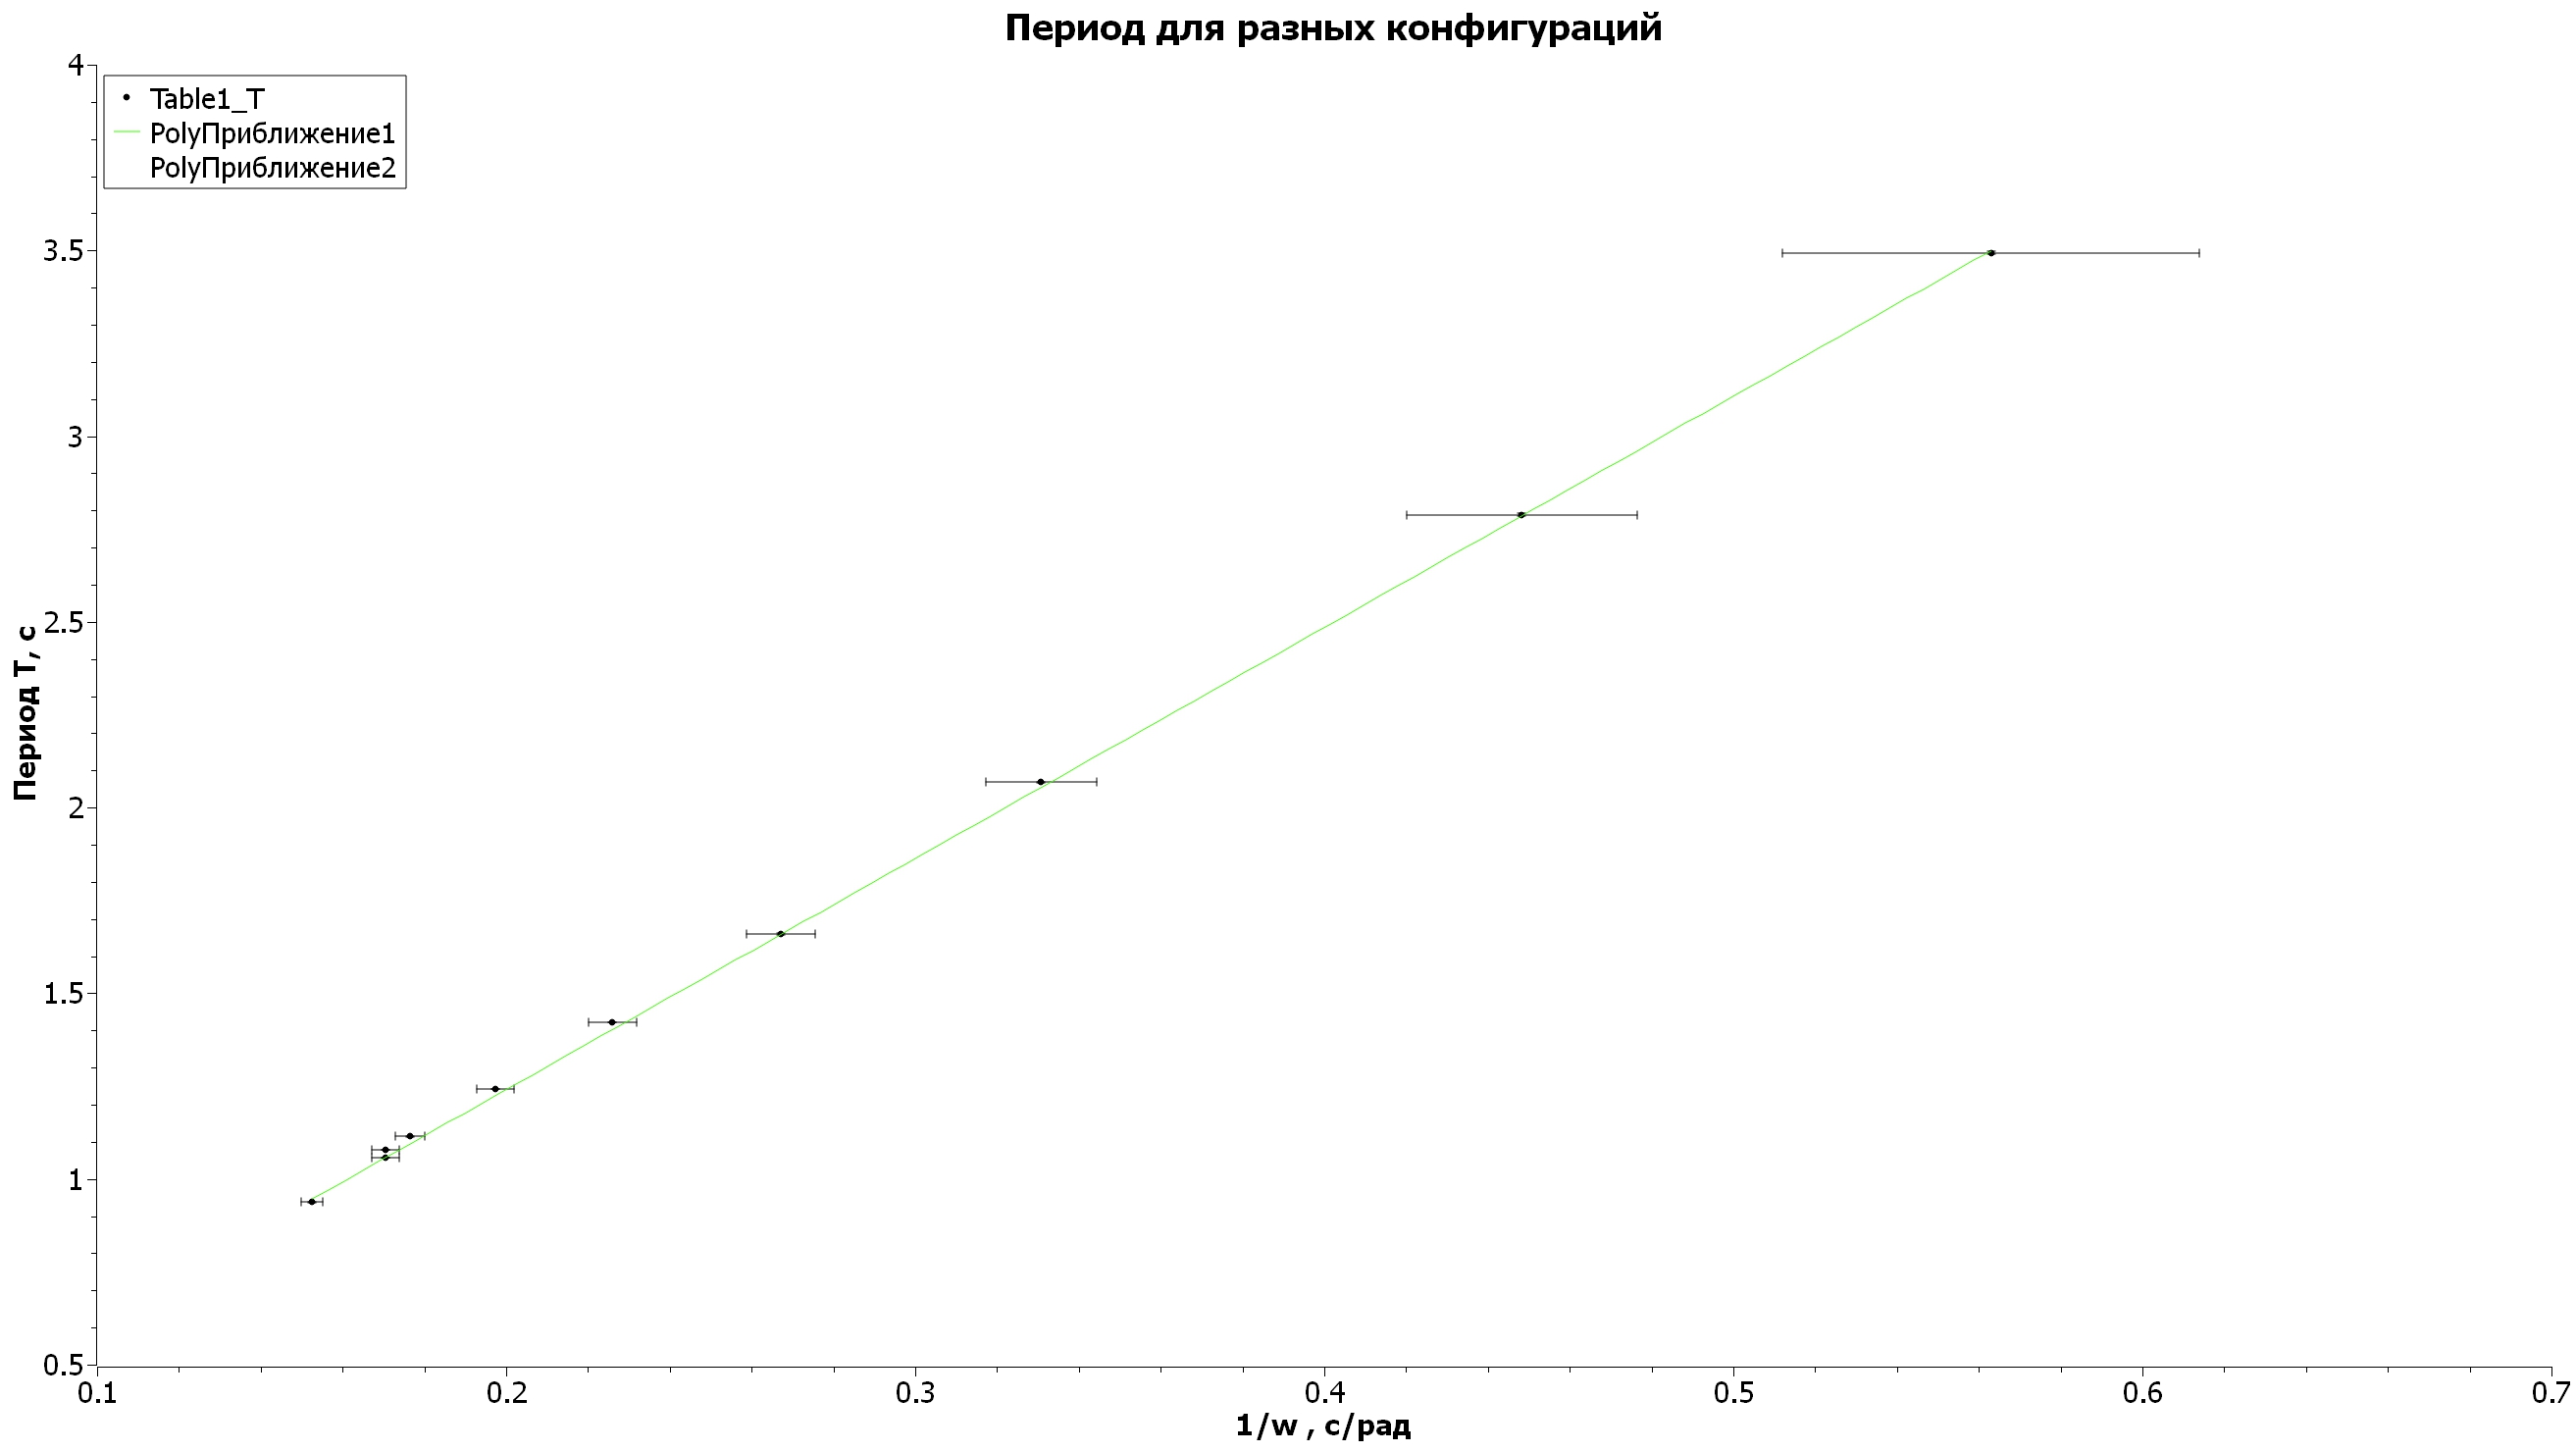
\includegraphics[scale=0.45]{T(w^-1)}
\end{flushleft}

Как видно точки хорошо ложаться на прямую, а угловой коэффициент $(6.2219\pm0.0013)$рад очень близок к теоретическим $2\pi$.

Для определения степени в зависимости периода от амплитуды построим график в логарифмических осях
\begin{flushleft}
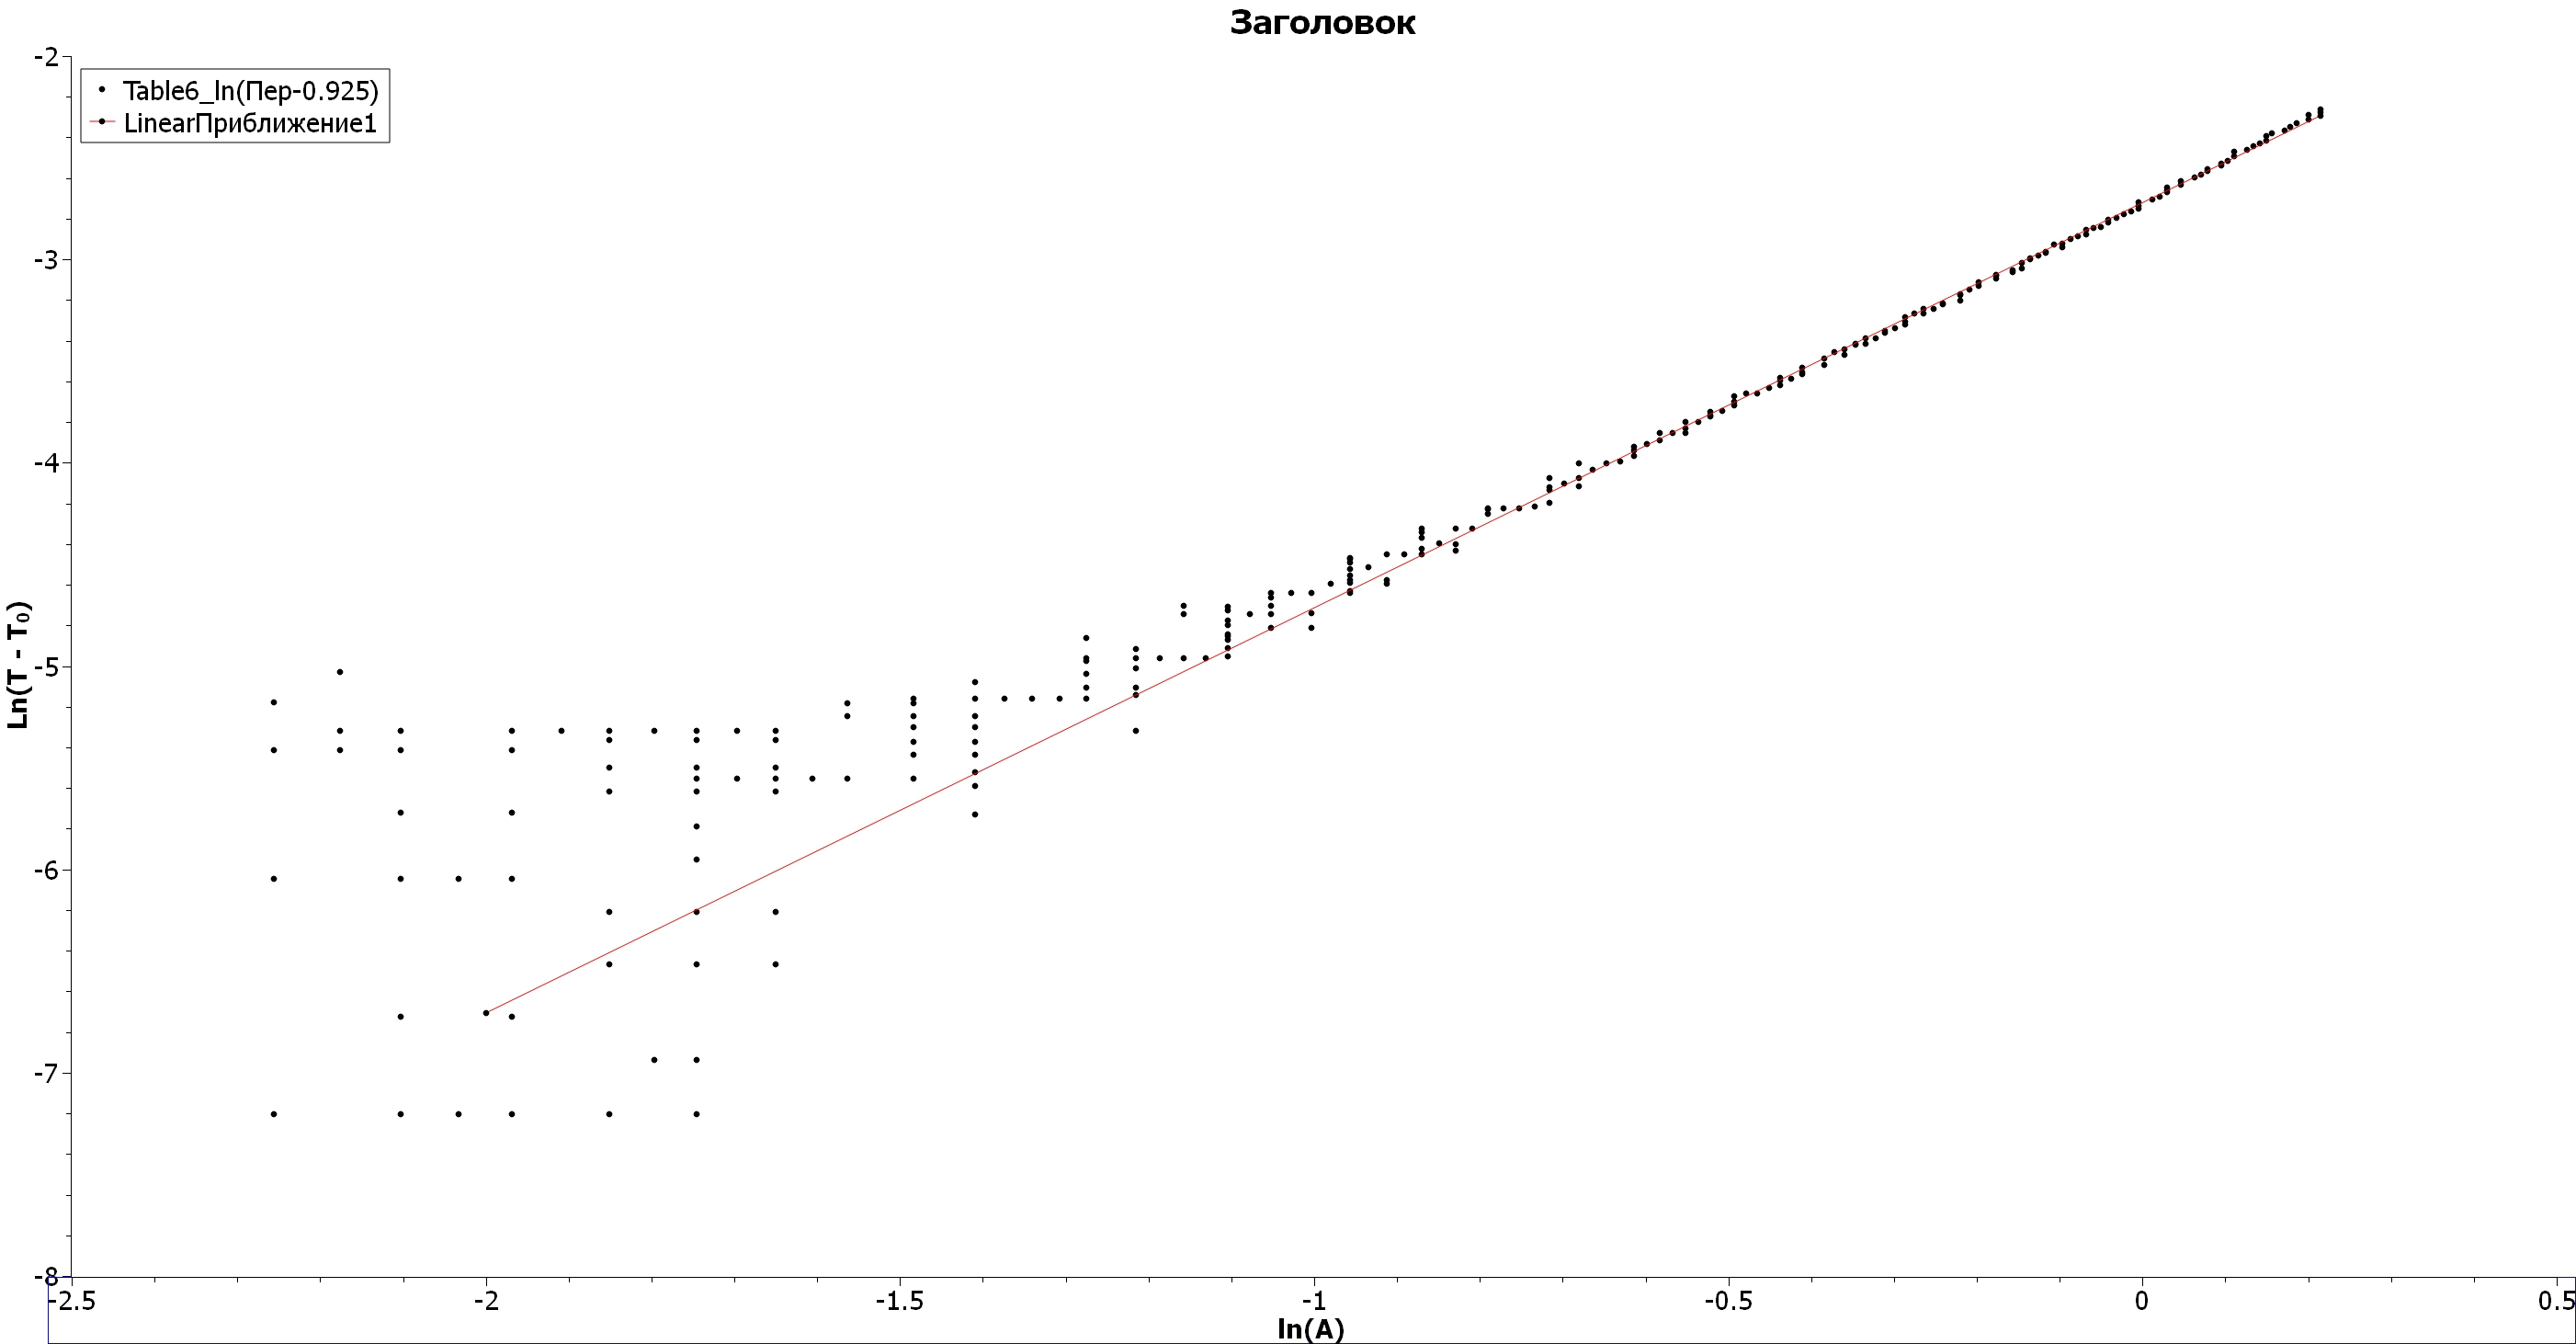
\includegraphics[scale=0.45]{Ln}
\end{flushleft}
Угловой коэффициент 1.993 близок к 2, а так выглядит квадратичное приближение в исходных осях.
\begin{flushleft}
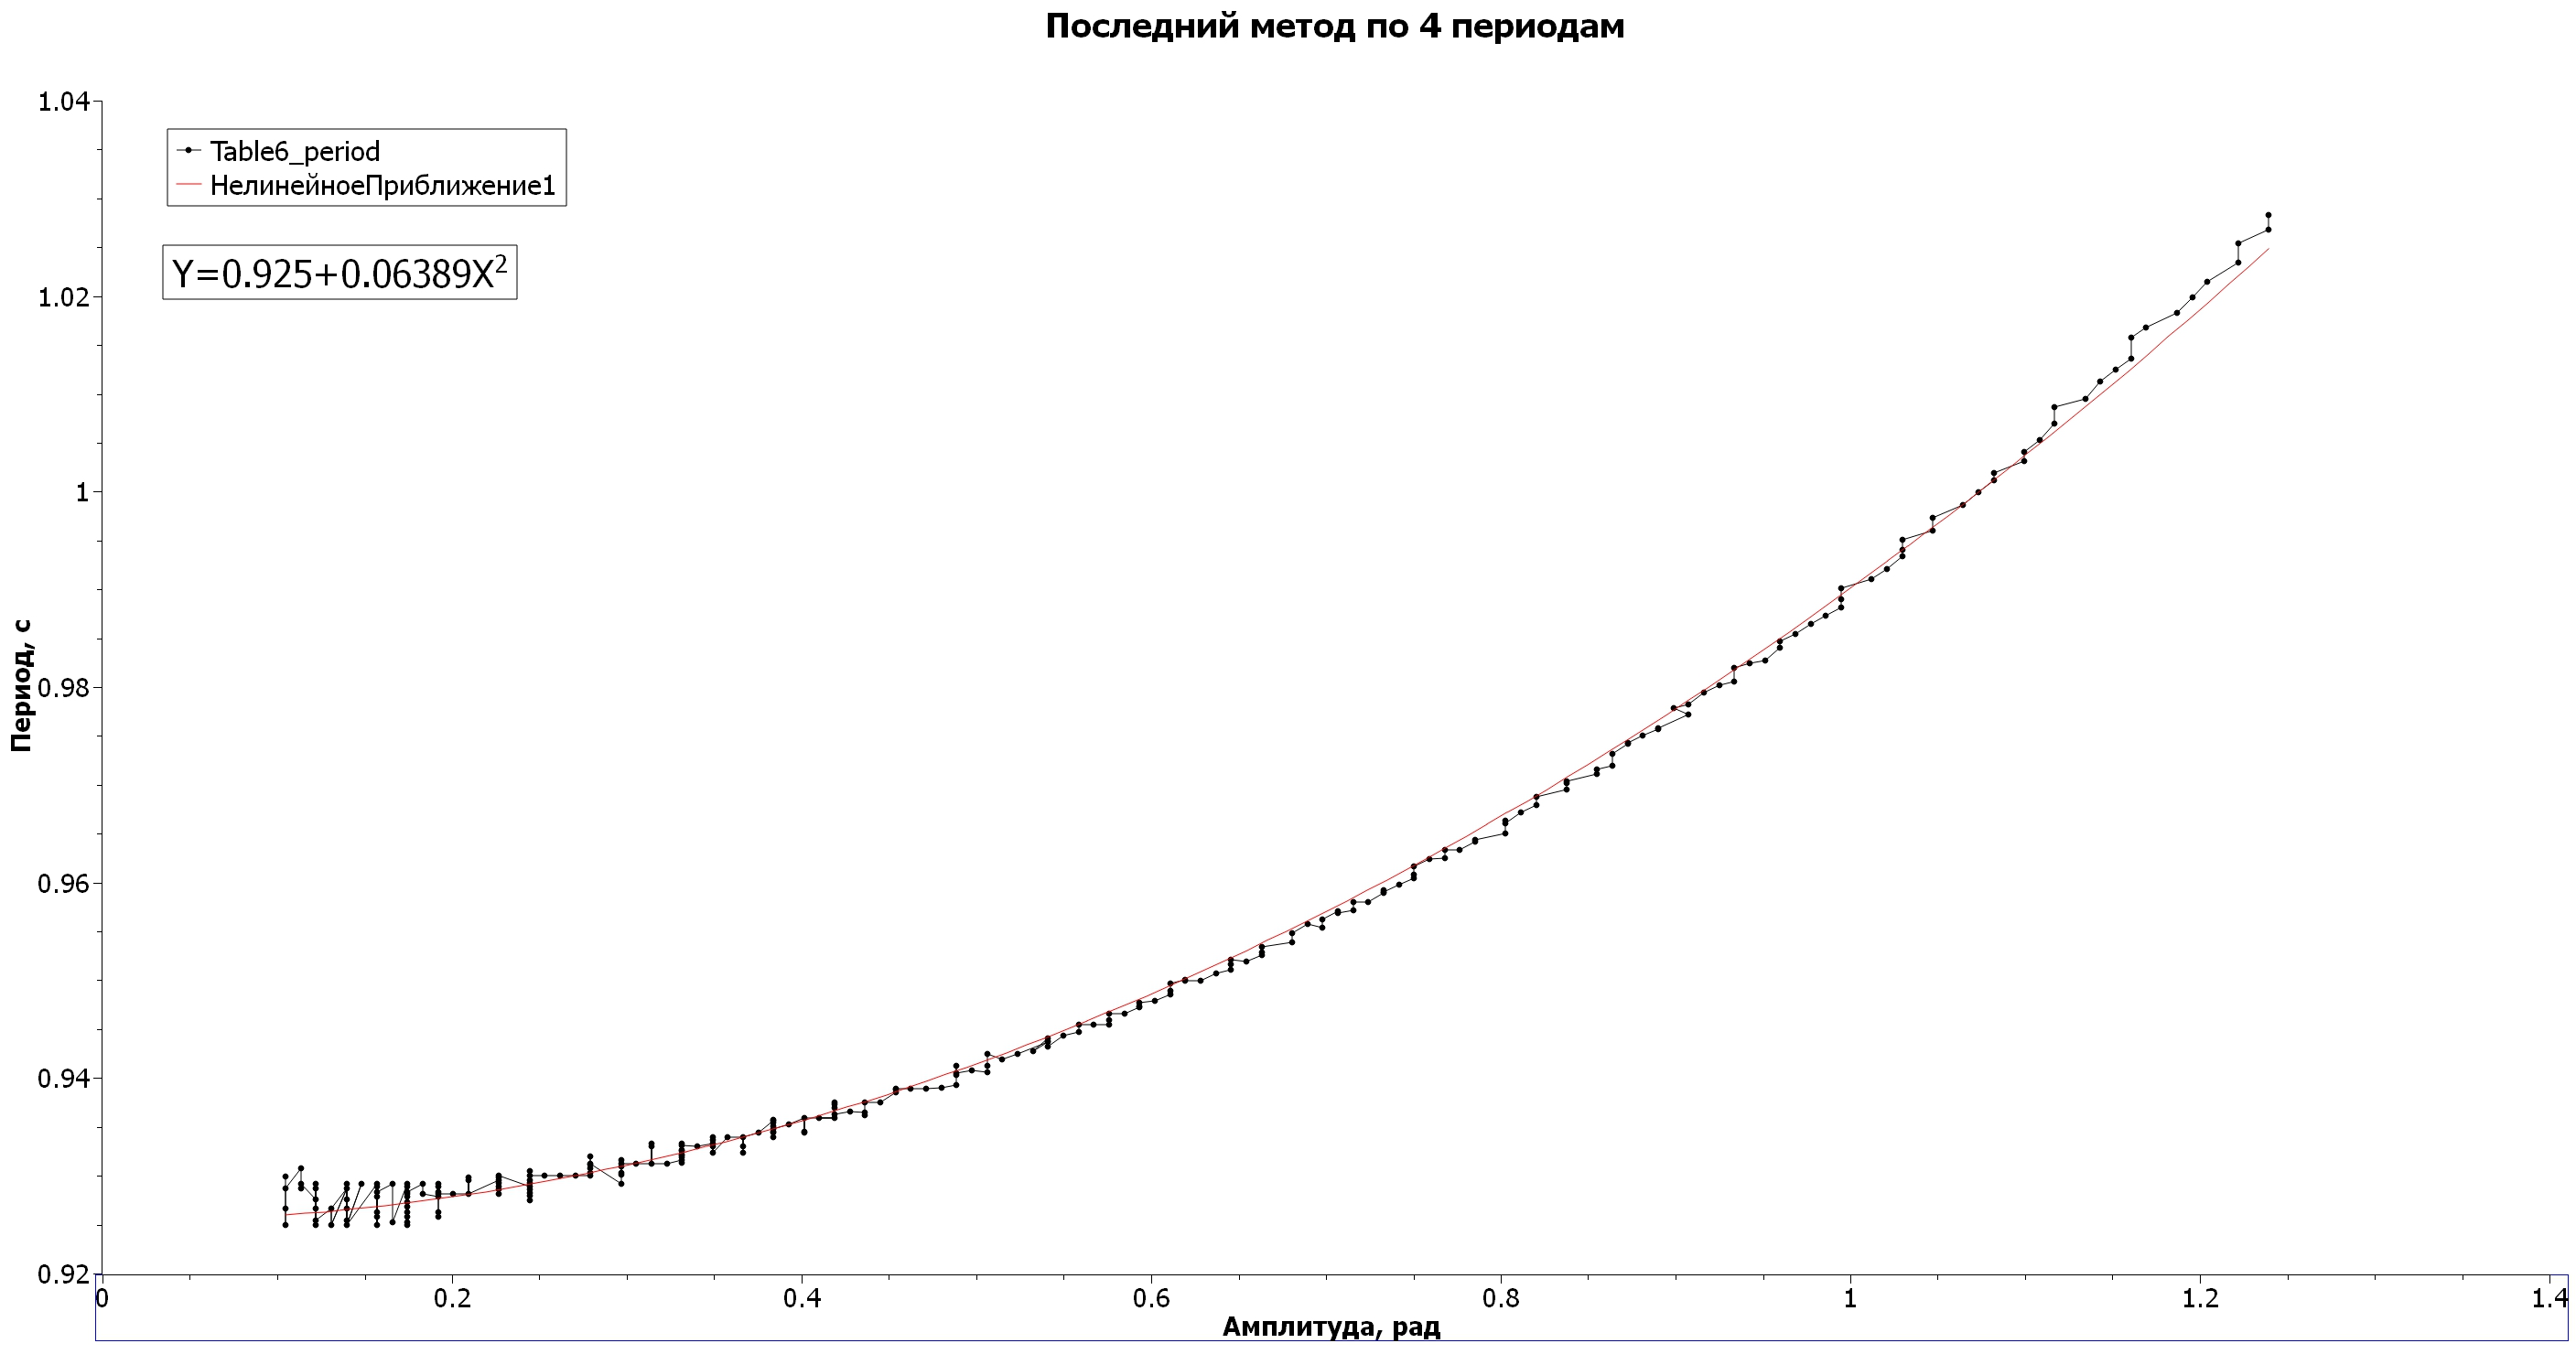
\includegraphics[scale=0.45]{T(A)}
\end{flushleft}

\end{document}
